\documentclass[12pt]{article}
\usepackage{titlesec}
\usepackage[utf8]{inputenc}
\usepackage[a4paper, total={6.5in, 9.5in}]{geometry}
\usepackage{fancyhdr}
\usepackage{graphicx} 
\usepackage{lipsum} 
\usepackage{tikz}
\usepackage{wrapfig}
\usepackage{acronym}
\usepackage{float}
\usepackage{siunitx}
\usepackage{multicol}
\usepackage{multirow}
\usepackage{pgfplots}
\usepackage{bm}
\usepackage{circuitikz}
\usetikzlibrary{shapes.geometric}
\usepackage{caption}
\usepackage{amsmath,amssymb,amsfonts}
\usepackage{cleveref}
\usepackage{algorithmic}
\usepackage{textcomp}
\usepackage{pdfpages}
\usepackage{xcolor}
\usepackage[numbers]{natbib}
\usepackage{listings}

\bibliographystyle{ieeetran}

\pgfplotsset{compat=1.18}
\usepackage{url}

% Page headers and footers
\pagestyle{fancy}
\fancyhf{}
\rhead{230155J}
\lhead{\textit{EN3551} - Assignment 02}
\cfoot{\thepage}

% MATLAB code formatting
\lstdefinestyle{mymatlab}{
    language=Matlab,
    backgroundcolor=\color{black!5},   
    basicstyle=\ttfamily\small,        
    keywordstyle=\color{blue}\bfseries,
    stringstyle=\color{purple},
    commentstyle=\color{green!50!black}\itshape,
    numbers=left,                      
    numberstyle=\tiny\color{gray},
    stepnumber=1,
    frame=single,                      
    breaklines=true,                   
    showstringspaces=false
}
\begin{document}

% Cover Page
\begin{titlepage}
    \centering
    \vspace*{0.5cm}
    
\includegraphics[width=5cm]{logo.png}
    \par\vspace{0.02cm}
    
    \textsf{\Large Department of Electronic \& Telecommunication Engineering,\\
    University of Moratuwa, Sri Lanka.}
    
    \vspace{2cm}
    {\LARGE\bfseries {Assignment 2 } \par}
    \vspace{1cm}

    {\large {Application of 2D-DCT for Image Compression}}

    \vspace{5.5cm}
  
    
        230155J - Dissanayake D. M. D. P. \\
        EN3551 - Digital Signal Processing \\
  
    
    \vspace{1.0cm}
    Date: \today
    \vfill



\end{titlepage}
%------------------------------------------------
%------------------------------------------------

\newpage

\section*{3.1 Comparison of Original and Reconstructed Images}
\subsection*{Barbara Image}

\begin{figure}[H]
    \centering
    \begin{minipage}{0.45\textwidth}
        \centering
        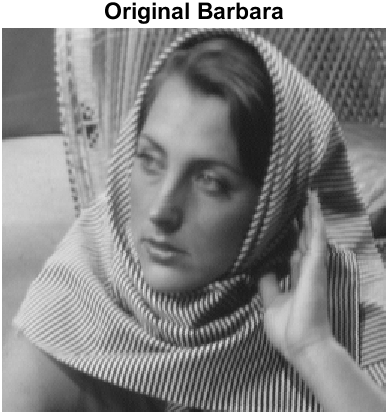
\includegraphics[width=0.8\linewidth]{barbara_original.png}
        \caption*{Original Image}
    \end{minipage}\hfill
    \begin{minipage}{0.45\textwidth}
        \centering
        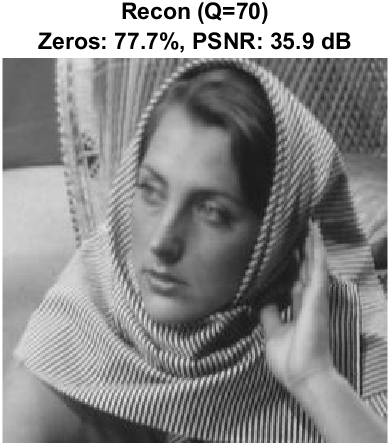
\includegraphics[width=0.8\linewidth]{barbara_reconstructed.png}
        \caption*{Reconstructed Image (Q70)}
    \end{minipage}
    \caption{Comparison of Original and Reconstructed Barbara Image}
\end{figure}

\textbf{Discussion:} The reconstructed Barbara image at Q70 retains most of the original details and there is minimal artifacts in sharp details. The edges and textures are well preserved effective compression without significant loss of quality. PSNR is 35.9dB indicating a better reconstruction.


\subsection*{Boats Image}

\begin{figure}[H]
    \centering
    \begin{minipage}{0.45\textwidth}
        \centering
        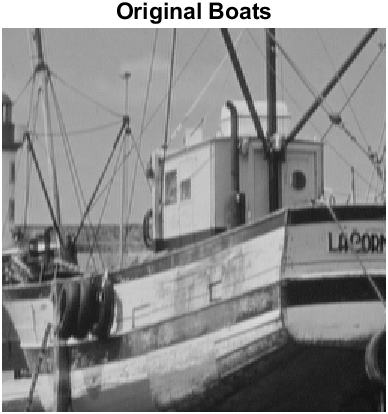
\includegraphics[width=0.8\linewidth]{boats_original.png}
        \caption*{Original Image}
    \end{minipage}\hfill
    \begin{minipage}{0.45\textwidth}
        \centering
        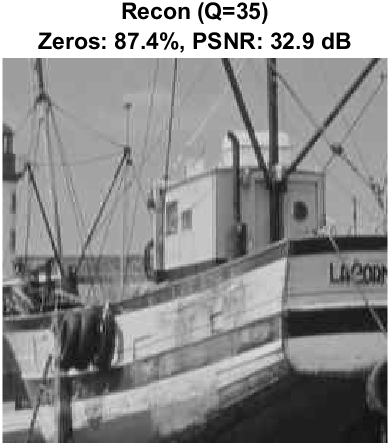
\includegraphics[width=0.8\linewidth]{boats_reconstructed.png}
        \caption*{Reconstructed Image (Q35)}
    \end{minipage}
    \caption{Comparison of Original and Reconstructed Boats Image}
\end{figure}

\textbf{Discussion:} The reconstructed Boats image at Q35 shows a noticeable loss of detail compared to the original. While the overall structure is maintained. But the finer textures and edges are blurred. This can be explained by the percentage of zeroes per 8x8 block which is about 87.4\%. The PSNR of the reconstructed image is 32.9dB and this confirms the slight difference that can be seen visually.

\subsection*{Peppers Image}

\begin{figure}[H]
    \centering
    \begin{minipage}{0.45\textwidth}
        \centering
        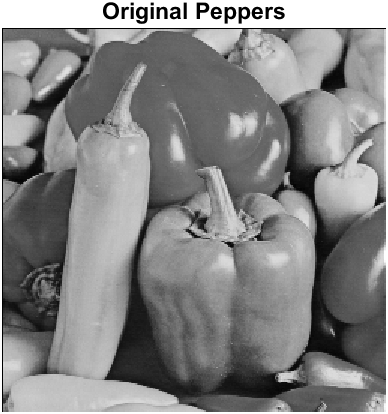
\includegraphics[width=0.8\linewidth]{peppers_original.png}
        \caption*{Original Image}
    \end{minipage}\hfill
    \begin{minipage}{0.45\textwidth}
        \centering
        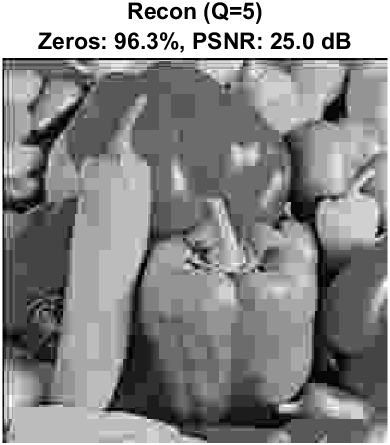
\includegraphics[width=0.8\linewidth]{peppers_reconstructed.png}
        \caption*{Reconstructed Image (Q5)}
    \end{minipage}
    \caption{Comparison of Original and Reconstructed Peppers Image}
\end{figure}

\textbf{Discussion: } The reconstructed Peppers image at Q5 shows significant loss of detail and quality. The image appears blurry and square like blocks are clearly vissible. At this low quality level it results in a high percentage of zeroes per 8x8 block (about 96.3\%). The compression is effective in reducing file size but the visual quality is compromised.The PSNR value is below 30dB so the structures of the reconstructed image is not preserved well and it can be seen by the human eye.
\subsection*{Sigiriya Image (Additional Image)}

\begin{figure}[H]
    \centering
    \begin{minipage}{0.47\textwidth}
        \centering
        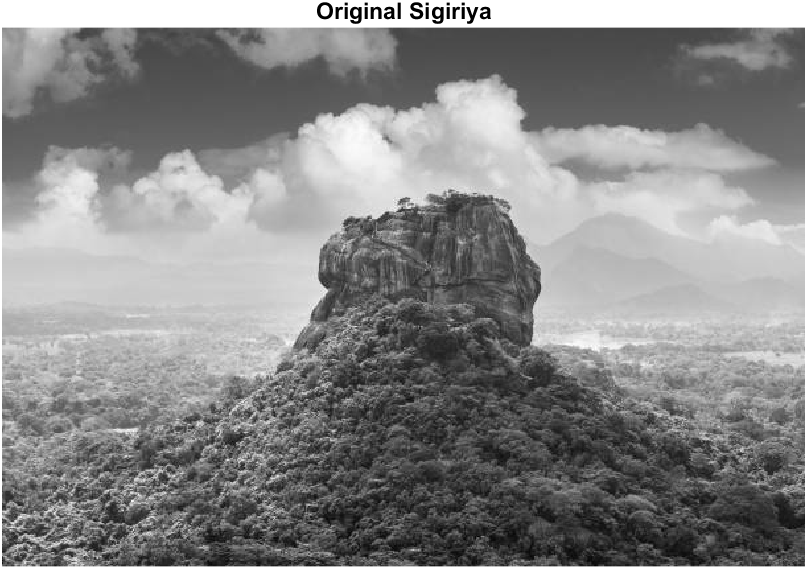
\includegraphics[width=1\linewidth]{sigiriya_original.png}
        \caption*{Original Image}
    \end{minipage}\hfill
    \begin{minipage}{0.47\textwidth}
        \centering
        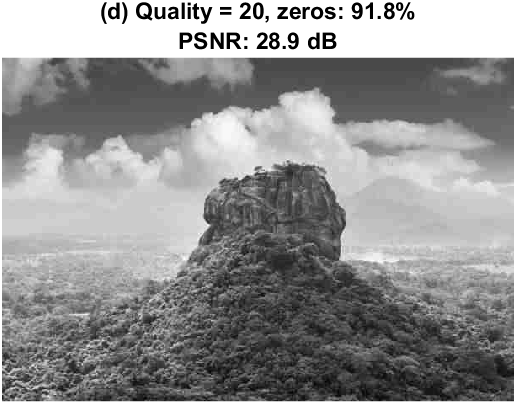
\includegraphics[width=1\linewidth]{sigiriya_reconstructed.png}
        \caption*{Reconstructed Image (Q20)}
    \end{minipage}
    \caption{Comparison of Original and Reconstructed Sigiriya Image}
\end{figure}
\textbf{Discussion: } The reconstructed image at 20\% quality level shows very little visual differences compared to the original image.Percentage of zeroes is 91.8\%. Sharp and high frequency content like trees and corners are somewhat affected, but the overall image is not much affected. This may be due to the higher height and width of image (608 * 408 \text{px})


\subsection*{Sweeping Different Quality Levels for Sigiriya Image}
\begin{figure}[H]
    \centering
    \begin{minipage}{0.45\textwidth}
        \centering
        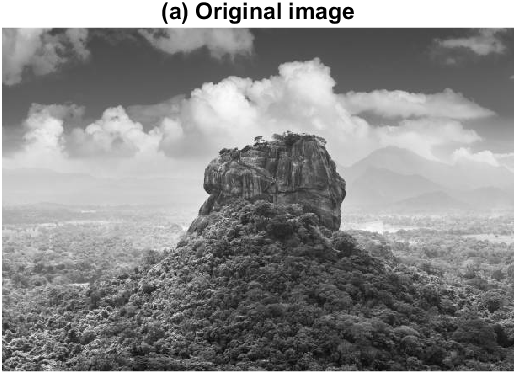
\includegraphics[width=0.8\linewidth]{sigiriya_original_.png}
        \caption*{Original Image }
    \end{minipage}\hfill
    \begin{minipage}{0.45\textwidth}
        \centering
        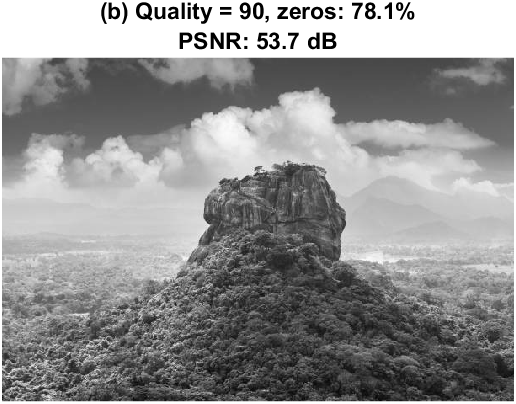
\includegraphics[width=0.8\linewidth]{sigiriya_90.png}
        \caption*{Reconstructed Image (Q90)}
    \end{minipage}
    
    
    \begin{minipage}{0.45\textwidth}
        \centering
        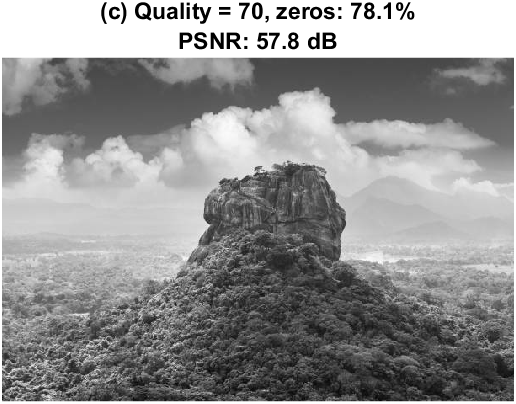
\includegraphics[width=0.8\linewidth]{sigiriya_70.png}
        \caption*{Reconstructed Image (Q70)}
    \end{minipage}\hfill
    \begin{minipage}{0.45\textwidth}
        \centering
        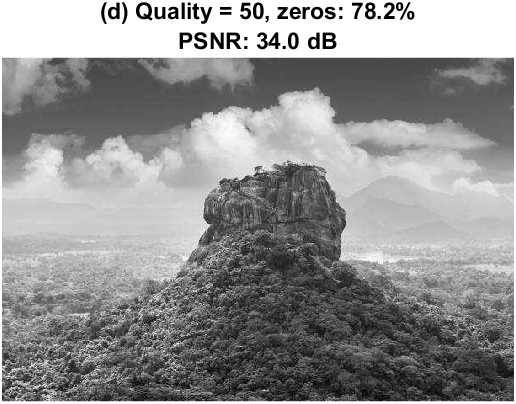
\includegraphics[width=0.8\linewidth]{sigiriya_50.png}
        \caption*{Reconstructed Image (Q50)}
    \end{minipage}


    \begin{minipage}{0.45\textwidth}
        \centering
        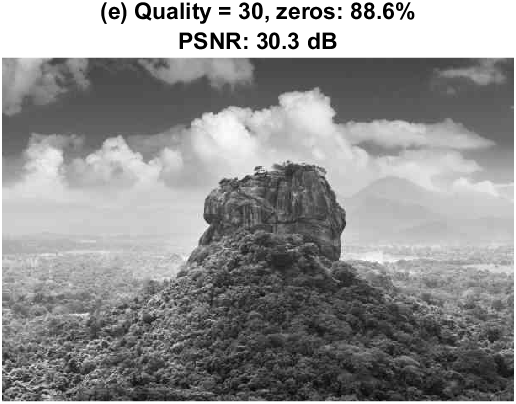
\includegraphics[width=0.8\linewidth]{sigiriya_30.png}
        \caption*{Reconstructed Image (Q30)}
    \end{minipage}\hfill
    \begin{minipage}{0.45\textwidth}
        \centering
        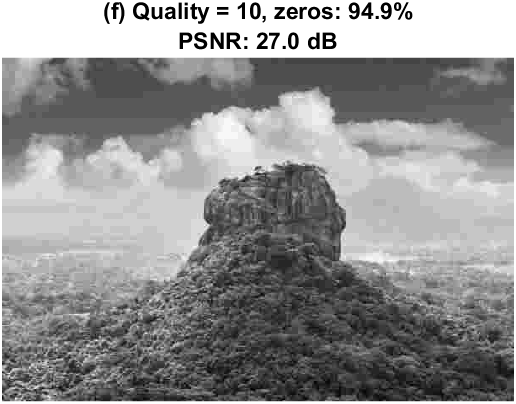
\includegraphics[width=0.8\linewidth]{sigiriya_10.png}
        \caption*{Reconstructed Image (Q10)}
    \end{minipage}
    
    
    \begin{minipage}{0.45\textwidth}
        \centering
        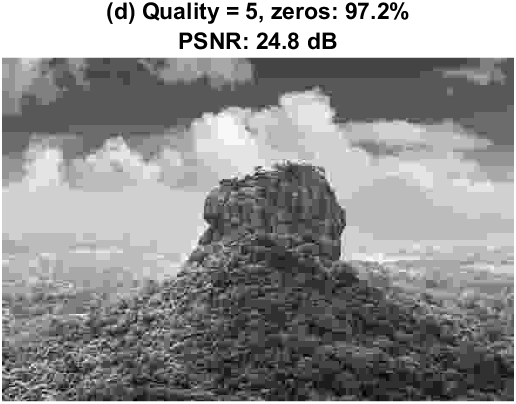
\includegraphics[width=0.8\linewidth]{sigiriya_5.png}
        \caption*{Reconstructed Image (Q5)}
    \end{minipage}\hfill
    \begin{minipage}{0.45\textwidth}
        \centering
        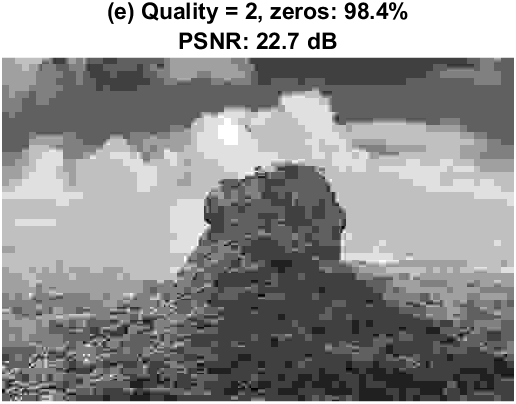
\includegraphics[width=0.8\linewidth]{sigiriya_2.png}
        \caption*{Reconstructed Image (Q2)}
    \end{minipage}

    \caption{Comparison of Reconstructed Sigiriya Images at Different Quality Levels}

\end{figure}

\subsubsection*{3.4 Discussion on the Effect of Quality Levels on different Images and compression}
The quality level in image compression using 2D-DCT significantly affects the reconstructed visual quality. Higher quality levels retain more of the original image's details and textures.It results in a reconstructed image that closely resembles the original. Conversely, lower quality levels (e.g., Q5) lead to more aggressive quantization, which can introduce artifacts and loss of fine details, making the reconstructed image appear blurry or pixelated.    

\begin{itemize}
    \item Images with high frequency content are difficult to compress without losing quality due to the sharp transitions like edges and textures. After compression these fine details can be blurred or pixelated.
    \item Plain images with not significant transistions like edges and textures can be compressed without pixelation. So these images can be considered as easier to compress. As an example, the Sigiriya Image has \textbf{sky and clouds} which are well presereved at lower qualities but the sharp detials in {trees and textures in rock} are visibly pixelated at very lower quality levels.
    \item The percentage of zeroes per 8x8 block is a good indicator of the compression level. Higher percentages indicate more aggressive compression, which can lead to loss of detail and visual similarity. The Peppers image at Q5 has a high percentage of zeroes (96.3\%) which results in significant loss of quality at least on plain surfaces.
\end{itemize}
\clearpage
\appendix
\section*{Appendix A: MATLAB Implementation}


\begin{lstlisting}[style=mymatlab, caption={Sample MATLAB script for 2D-DCT image compression}, label={lst:dct-compression}]
%% Load the data
barbara_data  = load('Images/barbara.mat');
boats_data    = load('Images/boats.mat');
peppers_data  = load('Images/peppers.mat');
sigiriya_data = load('Images/sigiriya.mat');

% Get the actual variable names
f_barb     = fieldnames(barbara_data);
f_boat     = fieldnames(boats_data);
f_pepp     = fieldnames(peppers_data);
f_sigiriya = fieldnames(sigiriya_data);

% Extract the images
barb_img     = barbara_data.(f_barb{1});
boat_img     = boats_data.(f_boat{1});
pepp_img     = peppers_data.(f_pepp{1});
sigiriya_img = sigiriya_data.(f_sigiriya{1});


% Convert colour to grayscale
if size(sigiriya_img, 3) == 3
    sigiriya_img = rgb2gray(uint8(sigiriya_img));
end


% Standard Q50 matrix (GIVEN)
Q50 = [16 11 10 16 24 40 51 61;
       12 12 14 19 26 58 60 55;
       14 13 16 24 40 57 69 56;
       14 17 22 29 51 87 80 62;
       18 22 37 56 68 109 103 77;
       24 35 55 64 81 104 113 92;
       49 64 78 87 103 121 120 101;
       72 92 95 98 112 100 103 99];

Q_barbara  = getQuantMatrix(Q50, 70);
Q_boats    = getQuantMatrix(Q50, 35);
Q_peppers  = getQuantMatrix(Q50, 5);
Q_sigiriya = getQuantMatrix(Q50, 30);

%% Evaluate the three test images + sigiriya
[recon_b, zeros_b, psnr_b] = evaluate_compression(barb_img,     Q_barbara);
[recon_o, zeros_o, psnr_o] = evaluate_compression(boat_img,     Q_boats);
[recon_p, zeros_p, psnr_p] = evaluate_compression(pepp_img,     Q_peppers);
[recon_s, zeros_s, psnr_s] = evaluate_compression(sigiriya_img, Q_sigiriya);

% Compare original vs reconstruction for the three test images
figure;
subplot(2,3,1); imshow(uint8(barb_img)); title('Original Barbara');
subplot(2,3,2); imshow(uint8(boat_img)); title('Original Boats');
subplot(2,3,3); imshow(uint8(pepp_img)); title('Original Peppers');
subplot(2,3,4); imshow(uint8(recon_b)); title(sprintf('Recon (Q=70)\nPSNR: %.1f dB', psnr_b));
subplot(2,3,5); imshow(uint8(recon_o)); title(sprintf('Recon (Q=35)\nPSNR: %.1f dB', psnr_o));
subplot(2,3,6); imshow(uint8(recon_p)); title(sprintf('Recon (Q=5)\nPSNR: %.1f dB', psnr_p));

% quality_levels = [90 70 50 30 10];

% figure('Name', 'Sigiriya - quality levels');
% subplot(2, 3, 1);
% imshow(uint8(sigiriya_img));
% title('(a) Original image');

% fprintf('\nSigiriya at different quality levels:\n');
% for k = 1:numel(quality_levels)
%     q = quality_levels(k);
%     Qk = getQuantMatrix(Q50, q);
%     [rec_k, zeros_k, psnr_k] = evaluate_compression(sigiriya_img, Qk);

%     fprintf('  Quality = %3d: Zeros = %.2f%%, PSNR = %.2f dB\n', q, zeros_k, psnr_k);
%     subplot(2, 3, k + 1);
%     imshow(uint8(rec_k));
%     title(sprintf('(%c) Quality = %d, zeros: %.1f%%\nPSNR: %.1f dB', ...
%           'a' + k, q, zeros_k, psnr_k));
% end

%DEFINING functions

function img = crop8(img)
    % Crop so both dimensions are multiples of 8
    [r, c] = size(img);
    img = img(1:floor(r/8)*8, 1:floor(c/8)*8);
end

function Q_new = getQuantMatrix(Q50, quality)
    if quality > 50
        tau = (100 - quality) / 50;
    elseif quality < 50
        tau = 50 / quality;
    else
        tau = 1;
    end

    Q_new = max(1, min(255, round(Q50 * tau)));
end

function [recon_img, percent_zeros, psnr_val] = evaluate_compression(orig_img, Q)
    orig_img = double(orig_img);
    [rows, cols] = size(orig_img);
    recon_img = zeros(rows, cols);
    total_elements = rows * cols;
    zero_count = 0;

    %STEP 1:
    % Perform DCT and quantization on each 8x8 block
    % Processing each 8x8 block
    for r = 1:8:rows
        for c = 1:8:cols
            block = orig_img(r:r+7, c:c+7);

            % Forward DCT and quantization
            C = dct2(block - 128);

        %STEP 2:
        
            S = round(C ./ Q);

            % Counting zeros in the quantized matrix
            zero_count = zero_count + sum(S(:) == 0);
            
            %STEP 4:
            % Perform inverse quantization and inverse DCT
            R = Q .* S;
            E = idct2(R);
            
            % Adding 128 to shift the pixel values back to the [0, 255] range
            recon_img(r:r+7, c:c+7) = E + 128;
        end
    end

    percent_zeros = (zero_count / total_elements) * 100;

    mse = sum((orig_img(:) - recon_img(:)).^2) / total_elements;
    if mse == 0
        psnr_val = Inf;
    else
        psnr_val = 10 * log10((255^2) / mse);
    end
end
\end{lstlisting}

\end{document}